% !TEX root = ../TensorOT.tex

%%% FIG %%%
\begin{figure}\centering
\begin{tabular}{@{}c@{}|@{}c@{}}
\includegraphics[width=.49\linewidth]{1d/cross-orient/linear-interp}&
\includegraphics[width=.49\linewidth]{1d/cross-orient/interp-ellipses}\\\hline
\includegraphics[width=.49\linewidth]{3d/plate-elong/linear-interp}&
\includegraphics[width=.49\linewidth]{3d/plate-elong/interp-ellipses}\\\hline
Linear interpolation & Quantum OT
\end{tabular}
\caption{Comparison of linear and quantum-OT interpolation (using formula~\eqref{eq-interpolating}). 
Each row shows a tensor field $\mu_t$ (top $d=2$, bottom $d=3$) along a linear segment from $t=0$ to $t=1$ ($t$ axis is vertical).
} \label{fig:1d-interp}
\end{figure}
%%% FIG %%%

%%% FIG %%%
\begin{figure}\centering
\begin{tabular}{@{}c@{}|@{}c@{}}
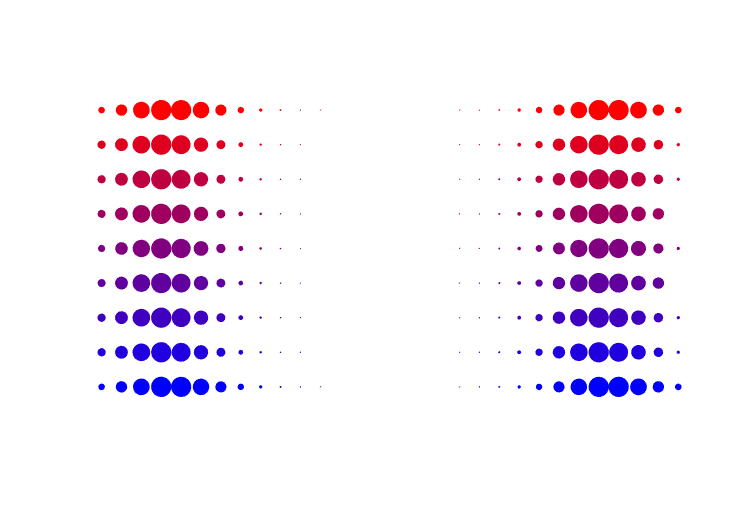
\includegraphics[width=.49\linewidth,trim=40 55 30 48,clip]{1d/dirac-pairs/interp-ot}&
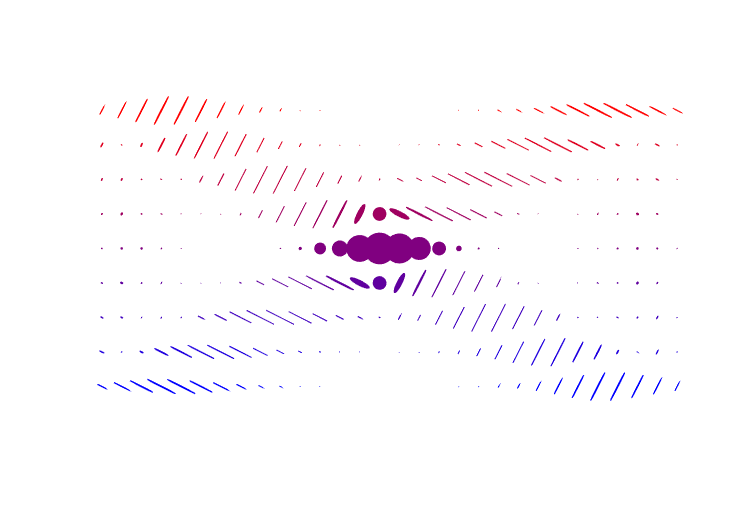
\includegraphics[width=.49\linewidth,trim=40 55 30 48,clip]{1d/dirac-pairs/interp-qot}\\\hline
Classical OT & Quantum OT
\end{tabular}
\caption{Comparison of classical OT (i.e. between isotropic tensors) and quantum-OT (between anisotropic tensors) interpolation (using formula~\eqref{eq-interpolating}), using the same display as Figure~\ref{fig:1d-interp}. 
} \label{fig:qot-vs-ot}
\end{figure}
%%% FIG %%%